\documentclass[compress,handout,10pt]{beamer}

\newlength{\wideitemsep}
\setlength{\wideitemsep}{\itemsep}
\addtolength{\wideitemsep}{100pt}
\let\olditem\item
\renewcommand{\item}{\setlength{\itemsep}{0.5\baselineskip}\olditem}

\usetheme{berlin}
\usecolortheme{beaver}
\usefonttheme[onlymath]{serif}

\usepackage{float}
\floatstyle{boxed}
\usepackage{colortbl}
\usepackage{mathpazo}
\usepackage{graphicx}
\usepackage{movie15}
\usepackage{bm}
\usepackage{verbatim}
\usepackage{comment}
\usepackage{caption}
\usepackage{subcaption}
\captionsetup[subfigure]{labelformat=empty}
\captionsetup[figure]{labelformat=empty}

\newcommand{\mygreen}{\color{green!50!black}}
\newcommand{\myblue}{\color{blue}}
\newcommand{\myred}{\color{red}}
\newcommand{\mycolor}{\color{red}{c}\color{blue}{o}\color{green}{l}\color{orange}{o}\color{cyan}{r}}
\newcommand{\mysize}{\scriptsize{s}\small{i}\normalsize{z}\Large{e}}
\newcommand{\myshape}{\textcircled{s}\textit{h}\texttt{a}\textsf{p}\textsc{e}}

\xdefinecolor{titlecolor}{rgb}{.855,.647,.125}
\setbeamercolor{frametitle}{fg=titlecolor}
\setbeamerfont{frametitle}{series=\bfseries}
\setbeamercolor{normal text in math text}{parent=math text}

\setbeamertemplate{navigation symbols}{} %gets rid of navigation symbols
\setbeamertemplate{footline}[frame number]
\beamertemplateshadingbackground{blue!5}{yellow!10}

\title{{\color{black} \LARGE Modeling and Simulating Fan Participation at Large Scale Sporting Events\newline} }

\subtitle{{\color{blue} \large Midterm Presentation} }

\author{ 
%    \vspace{5pt}
    {\bf{Presenter:}} \\ 
Steven Su \\ 
    \vspace{5pt}
} 
\institute{JHU AMS 550.400 Fall 2012}

\date{\mygreen Last Complied on \today} 

\begin{document}

\begin{frame}[plain]
    \titlepage
\end{frame}

\begin{frame}
    \frametitle{Overview}
    \tableofcontents
\end{frame}

\section{Introduction}

\subsection{Participants and Sponsors}

\begin{frame}
	\frametitle{Participants and Sponsors}
	\begin {itemize}
		\item Student participants:
			\begin {itemize}
				\item Steven Su
				\item Danni Tang
				\item Ahmed Aly
			\end {itemize}
		\item Sponsor: Blue Jays Unlimited	
	\end {itemize}
\end{frame}

\subsection{Sponsor Information}

\begin{frame}
    \frametitle{Who are Blue Jays Unlimited?}
    \begin {columns}
    	\begin{column}{0.5\textwidth}
    		\begin {itemize}
    			\item Blue Jays Unlimited (BJU) was established in 1995
    			\item Volunteer group of over 3000 alumni, friends and staff, based in Baltimore, MD, dedicated to supporting and promoting Johns Hopkins University (JHU) athletics
    			\item Official booster club for JHU athletics
    		\end {itemize}
    	\end {column}
    	\begin {column}{0.5\textwidth}
    		\begin{center}
    			
\includegraphics [width=2in] {BJU.jpg}
    		\end{center}
    	\end {column}
    \end{columns}
\end{frame}

\begin{frame}
	\frametitle{What Does BJU do for Hopkins?}
	\begin {columns}
		\begin {column} {0.5\textwidth}
			\begin {itemize}
				\item Raised more than \$4 million in funds to improve experience for JHU student athletes and fans alike
				\item Funds provide money for capital projects as well as scholarships and operational endowments
				\item Past projects include:
				\begin{itemize}
					\item Renovation of the Newton H.~ White Athletic Center
					\item Renovation of locker rooms
					\item Recognition banners for championship teams
				\end{itemize}
			\end {itemize}
		\end {column}
		\begin{column} {0.5\textwidth}
			\begin{center}
				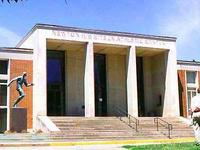
\includegraphics [width=2in] {AthleticCenter.jpg}
			\end{center}
		\end {column}
	\end {columns}
\end {frame}   

\begin{frame}
    \frametitle{BJU at Sporting Events}
    \begin{itemize}
    	\item BJU is present at nearly all major JHU sporting events
    	\item Encourage fans to cheer on their Blue Jays to victory in a vociferous and family-friendly manner
    	\item BJU's goal is to provide Hopkins' teams with the ultimate advantage: a spirited home crowd
    \end{itemize}
\end{frame}

\section{Problem Statement}

\subsection{Problem Statement Background}

\begin{frame}
	\frametitle{Problem Statement Background: Why is Cheering Important?}
		\begin{itemize}
			\item A loud and supportive home crowd is the ultimate hometeam advantage to any collegiate sports team 
			\item Fan participation in events such as chanting the school fight song, waving a rally towel, doing the wave,or general applause, show support for the home team as well as enhance the general atmosphere of a sporting event 
			\item Note that we will hence refer to all these activities as ``cheering''
		\end{itemize}
\end{frame}

\subsection{Official Problem Statement}

\begin{frame}
	\frametitle{Problem Statement}
			\begin {itemize}
				\item BJU is interested in maximizing cheering at Homewood Field located on the Homewood campus of JHU in Balitmore, MD. 
				\item BJU believes that they can increase cheering by placing ``cheer starters'' in the home crowd.
				\item ``Cheer starters'' are student volunteers who urge other fans around them to cheer. 
				\item BJU wants to know if ``cheer starters'' can actually increase cheering and also want a simple model of fan participation in cheering.
			\end {itemize}
\end{frame}

\section {Objectives}

\subsection{Important Details to Consider}

\begin{frame}
	\frametitle {Important Details To Consider}
		\begin {columns}
			\begin {column}{0.5\textwidth}
				\begin{itemize}
					\item Homewood Field's capacity is approximately 8500 spectators
					\item Long rectangular section of the bleachers in the lower left is traditionally reserved for Blue Jays' fans.
						\item Seats approximately 4000 fans
					\item Home bleachers are usually filled to capacity for all major Hopkins sporting events
				\end {itemize}
			\end {column}
			\begin {column}{0.5\textwidth}
				\begin{center}
    			
\includegraphics [width=2in] {BJU.jpg}
    		\end{center}
			\end {column}
		\end {columns}
\end{frame}

\subsection{Official Objectives}

\begin{frame}
	\frametitle {Official Objectives}
	\begin {itemize}
		\item Our task is to provide BJU with a simple model of fan participation in cheering at Homewood Field as well as simulation results from the model which determine if their belief about cheer starters is accurate. 
		\item If cheer starters are found to be effective, we will attempt to provide BJU more details about the quantity and location at which cheer starter should be placed in order to maximize cheering.
		\item Because of how fans normally sit, BJU is specifically interested in maximizing cheering in the home team bleachers.
	\end {itemize} 
\end{frame}

\section {Approach}

\subsection {Overview}

\begin {frame}
	\frametitle {Overview of Entire Model}
	\begin{itemize}
		\item Will create a model of a single fan and use this to simulate a large crowd.
		\item Single fan model will be stochastic in nature and will determine if a single fan starts to cheer
	\end{itemize}
\end {frame}

\subsection{Single Fan Model}

\begin {frame}
	\frametitle {A Model for a Single Fan: General Parameters}
	\begin{itemize}
		\item Stochastic model will use serveral parameters to determine whether a fan will participate in cheering
		\begin{itemize}
			\item Fan's innate level of support of the team
			\item Number of fans around a given fan who are cheering
		\end{itemize}
	\end {itemize}
\end {frame}

\begin {frame}
	\frametitle{A Model for a Single Fan: Fan's Innate Level of Support for Team}
	\begin{itemize}
		\item The greater the level of support a fan has for a team, the more likely he/she will cheer his/her team on.
		\item Model for single fan is stochastic in that the support level for the team will be randomized between fans
		\begin{itemize}
			\item Currently thinking of using a Normal Distribution (a bell curve) to randomly assign a score to represent a fan's innate support level.
			\item The majority of fans are average fans who go to games because they like the team. There are less fans which are fanatics for the team and less spectators who show up for the sporting event who don't care for the team.	
		\end{itemize}
		\item This more accurately reflects reality where different fans can have different levels of support for the same team.
	\end{itemize}
\end {frame}


\begin {frame}
	\frametitle {A Model for a Single Fan: Number of Fans Surrounding a Fan}
		\begin{itemize}
			\item The more people surrounding a fan who are cheering, the more likely the fan is likely to join the cheering.
			\item Will scale fan's innate support level score by number of surrounding fans who are cheering
			\item If total score exceeds pre-specified threshold, the fan will begin to cheer
		\end {itemize}
\end {frame}


	

%\section{Principles}
%\begin{frame}
%    \frametitle{Seven Basic Principles}
%     \begin{enumerate}
%         \item Set the context 
%         \item Choose effective examples and analogies
%         \item Choose vocabulary to suit your readers
%         \item Decide whether to present \#s in text, tables, or figures
%         \item Report and interpret \#s in the text
%         \item Specify the direction \emph{and} size of an association between variables
%         \item For many \#s, summarize overall pattern 
%     \end{enumerate}
%\end{frame}
%
%\section{Tools}
%\begin{frame}
%    \frametitle{Creating Effective Tables}
%\end{frame}
%
%\section{Arguments from Scale}
%
%\begin{frame}
%    \frametitle{Example: Cost of Packaging}
%\end{frame}
%
%\section{Graphical Methods}
%\begin{frame}
%    \frametitle{Example: The Nuclear Mission Arms Race}
%\end{frame}
%
%\section{Basic Optimization}
%\begin{frame}
%    \frametitle{Example: Maintaining Inventory}
%\end{frame}

\end{document}
